\section{Isolated Benzene}
\color{blue} 
    In order to verify if our new implementations work as intended, we compare the spectral functions we obtain for the isolated benzene ring with the one obtained by F. Hörbinger, via exact diagonalisation of the PPP model, in \cite{hoerbinger}. We find that our results shown in Fig. \ref{fig:isolated_benzene} match those from \cite{hoerbinger} up to three significant figures, after conversion into the appropriate units.
\color{black}

\medskip
\begin{figure}[!hbt]
    \centering
    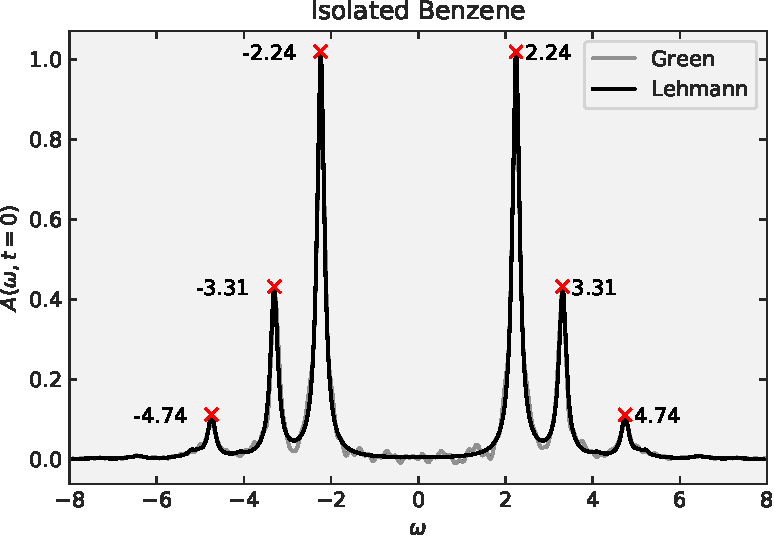
\includegraphics[width=0.7\textwidth]{graph/isolated_benzene.pdf}
    \caption{Spectral function of isolated benzene with peak energies in agreement with results form \cite{hoerbinger}\newline
    Parameters: $U = 3.96$, $a = 0.3$, $t_0 = 0$, broadening-factor $\epsilon = 0.1 $
    }\label{fig:isolated_benzene}
\end{figure}

\color{blue}
Fig. \ref{fig:isolated_benzene} also shows that both the Lehmann spectrum and the spectral function obtained via the Fourier transformation of the greens function produce comparable results
\color{black}